\documentclass[conference,compsoc,final,a4paper]{IEEEtran}
\usepackage[utf8]{inputenx}

%% Bitte legen Sie hier den Titel und den Autor der Arbeit fest
\newcommand{\autoren}[0]{Nockel, Sascha}
\newcommand{\dokumententitel}[0]{Das digitale Gedächtnis; warum Erinnern allein nicht ausreicht}

% Hie muss normalerweise nichts angepasst werden
\usepackage[pdftex]{graphicx}
\graphicspath{{img/}}
\DeclareGraphicsExtensions{.pdf,.jpeg,.jpg,.png}
\usepackage[cmex10]{amsmath}
\usepackage{algorithmic}
\usepackage{array}
\usepackage{dblfloatfix}
\usepackage{url}
\usepackage[autostyle=true,german=quotes]{csquotes}
\usepackage[backend=biber]{biblatex}
\usepackage{booktabs}
\usepackage{xcolor}
\usepackage{listings}             % Source Code listings
\usepackage[printonlyused]{acronym}
\usepackage{fancyvrb}
\usepackage[tocindentauto]{tocstyle} % Schönere Inhaltsverzeichnisse
\usetocstyle{allwithdot} % Punkte bei jedem Eintrag

% Farben definieren
\definecolor{linkblue}{RGB}{0, 0, 100}
\definecolor{linkblack}{RGB}{0, 0, 0}
\definecolor{darkgreen}{RGB}{14, 144, 102}
\definecolor{darkblue}{RGB}{0,0,168}
\definecolor{darkred}{RGB}{128,0,0}
\definecolor{comment}{RGB}{63, 127, 95}
\definecolor{javadoccomment}{RGB}{63, 95, 191}
\definecolor{keyword}{RGB}{108, 0, 67}
\definecolor{type}{RGB}{0, 0, 0}
\definecolor{method}{RGB}{0, 0, 0}
\definecolor{variable}{RGB}{0, 0, 0}
\definecolor{literal}{RGB}{31,0, 255}
\definecolor{operator}{RGB}{0, 0, 0}

\usepackage[ngerman]{betababel}
\usepackage[
      unicode=true,
      hypertexnames=false,
      colorlinks=true,
      colorlinks=false,
      linkcolor=darkblue,
      citecolor=darkblue,
      urlcolor=darkblue,
      pdftex
   ]{hyperref}
%	 \PrerenderUnicode{ü}

% Einstellungen für Quelltexte
\lstset{
    xleftmargin=0.1cm,
    basicstyle=\scriptsize\ttfamily,
    keywordstyle=\color{keyword},
    identifierstyle=\color{variable},
    commentstyle=\color{comment},
    stringstyle=\color{literal},
    tabsize=2,
    lineskip={2pt},
    columns=flexible,
    inputencoding=utf8,
    captionpos=b,
    breakautoindent=true,
    breakindent=2em,
    breaklines=true,
    prebreak=,
    postbreak=,
    numbers=none,
    numberstyle=\tiny,
    showspaces=false,      % Keine Leerzeichensymbole
    showtabs=false,        % Keine Tabsymbole
    showstringspaces=false,% Leerzeichen in Strings
    morecomment=[s][\color{javadoccomment}]{/**}{*/},
    literate={Ö}{{\"O}}1 {Ä}{{\"A}}1 {Ü}{{\"U}}1 {ß}{{\ss}}2 {ü}{{\"u}}1 {ä}{{\"a}}1 {ö}{{\"o}}1
}

\hypersetup{
    pdftitle={\dokumententitel},
    pdfauthor={\autoren},
    pdfdisplaydoctitle=true,
    hidelinks
}

% Makros für typographisch korrekte Abkürzungen
\newcommand{\zb}[0]{z.\,B.\ }
\newcommand{\dahe}[0]{d.\,h.\ }
\newcommand{\ua}[0]{u.\,a.\ }

% Wo liegt Sourcecode?
\newcommand{\srcloc}{src/}

% Literatur einbinden
\addbibresource{literatur.bib}
 % Weitere Einstellungen aus einer anderen Datei lesen

\begin{document}

% Titel des Dokuments
\title{\dokumententitel}

% Namen der Autoren
\author{
  \IEEEauthorblockN{\autoren}
  \IEEEauthorblockA{
    Hochschule Mannheim\\
    Fakultät für Informatik\\
    Paul-Wittsack-Str. 10,
    68163 Mannheim
    }
}

% Titel erzeugen
\maketitle
\thispagestyle{plain}
\pagestyle{plain}

% Eigentliches Dokument beginnt hier
% ----------------------------------------------------------------------------------------------------------

% Kurze Zusammenfassung des Dokuments
\begin{abstract}
Diese Arbeit gibt einen Überblick darüber was digitale Archive sind sowie über ihren grundlegenden Aufbau. Es wird betrachtet welche Probleme entstehen wenn digitale Daten auf lange Zeit archiviert werden sollen und wie man diesen entgegentreten kann. Es zeigt sich, dass aufgrund der speziellen Anforderungen an digitale Archive und der Lebensdauer für die sie ausgelegt sind, simple Dinge wie das Format der gespeicherten Daten eine enorme Rolle spielen und die damit einhergehenden Probleme nicht immer einfach zu lösen sind. In diesem Zusammenhang werden die beiden geläufigsten Methoden erläutert, um digitale Daten für die Zukunft zu konservieren und nutzbar zu halten.

\end{abstract}

% Inhaltsverzeichnis erzeugen
{\small\tableofcontents}

% Abschnitte mit \section, Unterabschnitte mit \subsection und
% Unterunterabschnitte mit \subsubsection
% -------------------------------------------------------
\section{Einleitung}
Seit Menschen damit begonnen haben Wissen und Geschichten für folgende Generationen festzuhalten, sei es auf Steintafeln, Schriftrollen oder in Büchern, ist der Wissensvorrat der Menschheit stetig gewachsen. Dank diesem Wissensvorrat wird es uns heute ermöglicht, komplizierte Sachverhalte und bedeutende Errungenschaften großer Denker und Erfinder der Vergangenheit nachzuvollziehen und auf ihnen aufzubauen, ohne jedes mal das \enquote{sprichwörtliche Rad} neu zu erfinden.

All dieses Wissen, genauer die Medien auf denen es festgehalten ist, muss irgendwo gelagert und verwaltet werden, da es niemandem von Nutzen ist wenn man nicht finden kann wonach man sucht. So ist schon in der Antike das wohl bekannteste Archiv der Welt entstanden, die Bibliothek von Alexandria \autocite{BibAlexAntike}. Heutige Archive und Bibliotheken bestehen noch immer zu großen Teilen aus analogen Medien wie Büchern oder Zeitschriften. Seit dem Beginn des Zeitalters der Digitalisierung werden diese jedoch immer mehr von digitalen Datenträgern wie CDs, Festplatten oder Magnetbändern abgelöst, da sie im Vergleich zu einem Buch bei gleichem oder geringerem Platzbedarf eine vielfach größere Menge an Daten speichern können \autocite{KLA2015}. So ist die auf Amazon erhältliche deutsche eBook Ausgabe des Silmarillion von J.R.R. Tolkien ca. 2 \ac{MB} groß, während beispielsweise handelsübliche Festplatten mit Kapazitäten von hunderten \ac{GB} bis hin zu mehreren \ac{TB} erhältlich sind. Auf einer Festplatte mit 3 \ac{TB} Kapazität können also bei dem physikalischen Platzbedarf eines Taschenbuches schon ca. 1,5 Millionen eBooks untergebracht werden.

Nicht nur wegen der effizienteren Speicherung der Daten, sondern auch wegen der Möglichkeit des schnelleren und einfacheren Auffindens der gesuchten Inhalte setzen Bibliotheken und Archive schon lange auf digitale Datenhaltung zusätzlich zu ihrem normalen Angebot \autocite{KLA2015}. Da das globale Datenaufkommen voraussichtlich auch in Zukunft weiter steigen wird, werden auch digitale Archive immer mehr an Bedeutung gewinnen \autocite{Reinsel2018}.

Diese Arbeit soll einen Überblick darüber geben, was ein digitales Archiv ausmacht sowie die Frage beantworten, wieso das alleinige Speichern von Daten nicht ausreicht, um dem Anspruch gerecht zu werden, Wissen für künftige Generationen zu erhalten. Da das Thema nahezu alle Bereiche der Informatik berührt wird in Kapitel 2 zunächst ein Grundverständnis darüber vermittelt weshalb man digitale Archive benötigt, welche Anforderungen an sie gestellt und wie sie letztendlich realisiert werden können. Das Hauptaugenmerk der Betrachtungen liegt hierbei auf Archiven, welche Daten auf mittel- bis langfristige Sicht speichern.

In Kapitel 3 geht es darum, welche Probleme bei der langfristigen Speicherung von Daten in Archivsystemen im Zusammenhang mit den Anforderungen an ein solches System bestehen. Kapitel 4 erläutert schließlich die zwei am weitesten verbreiteten Techniken zur Lösung der in Kapitel 3 beschriebenen Probleme und Kapitel 5 gibt eine kurze Zusammenfassung dieser Betrachtung, sowie eine Antwort auf die Forschungsfragen.

% -------------------------------------------------------
\section{Digitale Archive}
Digitale Archive bieten viele Vorteile im Vergleich zu ihren analogen Vorfahren, deshalb stellen sie jedoch auch andere Anforderungen und sind mitunter sehr komplex. Anders als für analoge Speichermedien, wie Bücher, wird immer eine Infrastruktur aus Hard- und Software benötigt um ein solches Archiv zu betreiben.

% -----------------------------
\subsection{Anwendungsbereiche}
Digitale Archive finden eine weite Verbreitung, denn überall wo digitale Daten anfallen, ist es potenziell gewünscht diese auf lange Zeit zu speichern. Dies kann im kleinen Rahmen mit der privaten Foto- und Videosammlung oder im größeren wie zum Beispiel bei Firmen stattfinden, die in Deutschland laut Abgabenordnung (AO) § 147 auch gesetzlich dazu verpflichtet sind einen Großteil ihrer Akten auf mehrere Jahre und im Fall von medizinischen Daten, nach dem Bürgerlichen Gesetzbuch (BGB) § 852, sogar Jahrzehnte zu archivieren, für den Fall dass Schadenersatzansprüche aufgrund fehlerhafter Behandlung geltend gemacht werden.

Die Art der gespeicherten Daten in digitalen Archiven ist je nach Anforderung ganz unterschiedlich. So werden etwa im deutschen Bundesarchiv ausschließlich Sachakten archiviert \autocite{Berger2005}. Das deutsche Satellitendatenarchiv (\acs{D-SDA}), welches vom deutschen Zentrum für Luft- und Raumfahrt betrieben wird, archiviert dagegen ausschließlich Daten, die bei Missionen zur Erdbeobachtung anfallen \autocite{Memishi2019}. Dies sind Beispiele für spezialisierte Archive, jedoch gibt es auch Archive die ein breiteres Spektrum an Daten beinhalten. Das gemeinnützige Internet Archive Project in San Francisco hat beispielsweise damit begonnen, Webseiten zu archivieren und mit der eigens entwickelten ``Wayback Machine'' abrufbar zu machen. Inzwischen beinhaltet das Internet Archive jedoch auch Bücher, Videos, Audioaufnahmen, Software und Bilder \autocite{AboutIA}.

% -----------------------------
\subsection{Anforderungen}
In der Regel stellen große Archive wie das deutsche Bundesarchiv oder das \acs{D-SDA} sehr individuelle Anforderungen an ihr jeweiliges Archivsystem. So kommt es nicht selten vor, dass die Archive speziell für ihre Bedürfnisse entwickelte Software verwenden, wie zum Beispiel das Bundesarchiv, welches die Eigenentwicklung BASYS-S-Oracle zur Erschließung der bereits erwähnten Sachakten verwendet. Für andere Daten wie Bilder oder Audioaufnahmen ist diese Software hingegen nicht geeignet \autocite{Berger2005}.

Bei der Anforderungsanalyse spielen viele Faktoren eine Rolle. So ist für eine Bibliothek die Benutzerfreundlichkeit der Archivsoftware meist von großer Wichtigkeit, während ein reines Archiv eher darauf bedacht ist Risiken für die Integrität und Sicherheit der Daten zu minimieren, was mithilfe von Replikationen und verschiedenen Redundanzmechanismen bei der Speicherung der Daten erreicht wird. Das Internet Archive betreibt aufgrund dieser Anforderung Spiegelserver in der neuen Bibliothek von Alexandria welche immer eine Kopie der Server in San Francisco bereithalten \autocite{BibAlexIAMirror}. Eine solche Risikominimierung ist natürlich mit erheblichen Kosten verbunden und deshalb nicht unbedingt für jedes Archiv von gleicher Wichtigkeit. Nicht nur an die Hardware, sondern auch an die Software werden wie der Fall des deutschen Bundesarchivs zeigt, je nach Einsatzgebiet besondere Anforderungen gestellt. Um systematisch eine Lösung für beide Bereiche zu erarbeiten gibt es verschiedene Methoden die sich bewährt haben. Eine davon ist der PLANETS Preservation Planning approach \autocite{Strodl2007}. Hier werden in Workshops mit Experten mehrere hierarchisch geordnete Möglichkeiten für die Umsetzung erarbeitet. Am Ende des Prozesses kann mathematisch eine Rangliste für die einzelnen Teilbereiche erstellt werden, auf deren Grundlage die Entscheidung für eine Lösung getroffen werden kann.

% -----------------------------
\subsection{Umsetzung}
Das \ac{OAIS} Referenzmodell, welches ursprünglich in der ISO 14721:2003 vorgestellt und 2012 in der ISO 14721:2012 noch einmal überarbeitet wurde, bietet eine konzeptionelle Anleitung für die Umsetzung eines digitalen Archivs. Das Informationsmodell nach \ac{OAIS} sieht es vor, dass alle Daten die durch das System fließen in Pakete gepackt werden.

Die drei Arten von Paketen sind \ac{SIP}, \ac{AIP} und \ac{DIP}. Die \ac{SIP}s sind hierbei der Einstieg der Daten in das Archivsystem, da in diesen Paketen Daten und Informationen enthalten sind die benötigt werden, um aus ihnen \ac{AIP}s zu erstellen, welche die Pakete sind die eigentlich im Archivsystem gespeichert werden. Die \ac{DIP}s sind wiederum Versionen von \ac{AIP}s die auf bestimmte Anforderungen der Nutzer oder anderer Systeme welche die Daten verwenden abgestimmt sind. 

\begin{figure}[!ht]
\centering
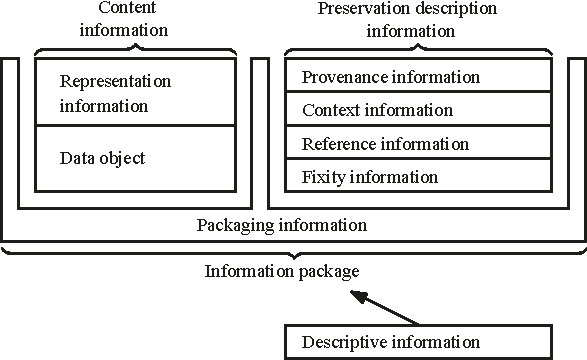
\includegraphics[width=8.3cm]{InformationPackageModel_Ball2006}
\caption{Information Package Model \autocite{Ball2006}}
\label{oais}
\end{figure}

Diese drei Pakettypen bestehen grundsätzlich aus zwei Blöcken, zum einen dem Block für die Inhaltsinformationen, der die eigentlichen Daten und die zugehörigen Metadaten enthält sowie dem \ac{PDI} Block. Der \ac{PDI} Block beinhaltet eine genaue Änderungshistorie für den Block der Inhaltsinformationen sowie Informationen über den Kontext in dem die Daten stehen und welche Referenzen zu den Daten vorhanden sind. Außerdem beinhaltet er auch Informationen über die Beständigkeit der Daten, wie etwa Prüfsummen um verifizieren zu können, dass die Daten nicht korrumpiert wurden. Diese beiden Blöcke umgeben die eigentlichen Paketinformationen die das Suchen und wieder Auffinden des Pakets ermöglichen und es identifizierbar machen sollen (vgl. \autoref{oais} auf Seite~\pageref{oais}) \autocite{Ball2006}.

Neben dem Aufbau der Informationspakete werden auch Verantwortlichkeiten beschrieben die ein \ac{OAIS} wahrnehmen sollte, um konform zu sein. Da die Norm jedoch nicht den Anspruch erhebt eine definitive Anleitung zur Implementierung eines solchen Systems zu sein, existieren gewisse Freiheitsgrade weshalb nicht alle Archivsysteme alle Punkte genau umsetzen \autocite{Ball2006}.

% -------------------------------------------------------
\section{Herausforderungen im Lebenszyklus von Archivdaten}
Die Daten in digitalen Archiven sind im Gegensatz zu den Daten in normalen Speichersystemen von gänzlich anderen Problemen betroffen als nur dem Ausfall der Speichermedien auf denen sie sich befinden. So werden in herkömmlichen Speichersystemen wie etwa einem \ac{NAS} die Daten in der Regel häufiger abgerufen oder verändert, wodurch indirekt Mechanismen wie zum Beispiel die Fehlerkorrektur des \ac{RAID} greifen und so die Daten im Falle einer fehlerhaften Prüfsumme automatisch über die Paritätsinformationen des \ac{RAID} wiederhergestellt werden \autocite{Lakshmi2008}. Dies ist bei Archiven in der Regel nicht der Fall, da Daten hier meist auf lange Sicht, mitunter sogar Jahrzehnte, nicht abgerufen werden, auch eine Veränderung der Daten ist in einem Archiv normalerweise nicht gewünscht. Der Verfall der gespeicherten Informationen ist jedoch nur ein kleiner Teil der Risiken und Probleme für Archivdaten der durch regelmäßige Maßnahmen wie das sogenannte ``data scrubbing'', bei dem alle Speicherblöcke auf Fehler geprüft und auftretende Fehler korrigiert werden, weitestgehend eliminiert werden kann \autocite{Lakshmi2008}. Aufgrund der Langlebigkeit von Archivdaten spielen auch ganz andere Faktoren eine Rolle die bei Daten in gebräuchlichen Systemen, die nur für einige Jahre ausgelegt sind, nicht von Bedeutung sind. Folgende drei Kategorien sind hier von besonderem Interesse.

% -----------------------------
\subsection{Neue Hard- und Software}
Kein Speichermedium ist unbegrenzt haltbar, das gilt besonders für Festplatten, die einen Großteil des Speichers zur Verfügung stellen der weltweit verwendet wird. Deswegen wurden Technologien wie \ac{RAID} entwickelt um Datenverluste zu verhindern und einen reibungslosen Austausch von defekten oder ausgedienten Festplatten zu ermöglichen \autocite{Lakshmi2008}. Auch Neuerungen in der Technik können einen Austausch der Speichermedien durch beispielsweise langlebigere oder über mehr Kapazität verfügende Hardware bedeuten. Es sind aber nicht nur Defekte an der Hardware die einen Datenverlust bedingen können, sondern auch die Software oder im Fall der Festplatten die Firmware die für die Verwaltung der physikalischen Speicherblöcke zuständig ist. Deshalb gilt es wie bei allen Softwaresystemen auch bei Archivsystemen die verwendete Software immer aktuell zu halten um eventuelle Fehler oder auch Sicherheitslücken zu beseitigen und einen sicheren Betrieb zu gewährleisten \autocite{Lakshmi2008}.

Der Austausch von Hardware und die Aktualisierung von Software bedeutet für die Archivdaten Veränderung, da die Daten vom auszutauschenden Speichermedium auf das neue migriert oder eventuell durch neue Software anders organisiert werden müssen. Weil Archive jedoch den Anspruch haben ihren Bestand möglichst originalgetreu zu speichern und zu konservieren, birgt jede Aktualisierung der Hard- oder Software das Risiko der Kompromittierung. Aus diesem Grund ist es besonders wichtig die Integrität, aber auch die Authentizität der Daten zu gewährleisten. Hierzu sieht das \ac{OAIS} vor allem die \ac{PDI} Blöcke vor, welche alle Veränderungen an den zugehörigen \ac{AIP}s dokumentieren sowie etwaige Informationen zur Sicherstellung der Integrität in Form von Prüfsummen enthalten.

% -----------------------------
\subsection{Unbeständigkeit von Dateiformaten}
Paradoxerweise stellen besonders Dateiformate ein großes Problem für digital archivierte Daten dar, das liegt vor allem daran, dass es nicht unbedingt garantiert werden kann, dass beispielsweise das archivierte Word 2003 Dokument auch in 100 Jahren noch geöffnet werden kann, da entweder keine Version von Word mehr verfügbar ist welche das Dokument öffnen kann oder die Software schlicht nicht mehr erhältlich ist, weil die Entwicklung eingestellt wurde oder die Firma nicht mehr existiert \autocite{dpcFormatsStandards}.

Open-Source-Dateiformate wie JPEG2000 bieten dagegen den Vorteil, dass sie von einer Vielzahl von Entwicklern am Leben gehalten und weiterentwickelt werden, weshalb sie sich im Gegensatz zu proprietären Formaten generell eher für ein Archivsystem eignen. Es ist aber längst nicht für jede Form von Daten ein passendes Open-Source-Format erhältlich, das gilt etwa für \ac{CAD} Dateitypen welche in der Regel von großen Konzernen entwickelt und gepflegt werden. So liegt die Verantwortung für die Pflege der Formate wieder bei den Konzernen, womit wiederum eine gewisse Unsicherheit für die Zukunft des Formats einhergeht \autocite{dpcFormatsStandards}. 

Deshalb ist es sinnvoll sich schon beim Planen eines Archivs genaue Gedanken darüber zu machen, welche Formate unterstützt werden sollen, da hierdurch die eventuell später folgende Migration auf neuere Versionen der verwendeten Formate stark vereinfacht, beziehungsweise erst ermöglicht wird \autocite{dpcFormatsStandards}.

Die Entscheidung für eine kleine Anzahl von verwendeten Formaten bedeutet unter Umständen jedoch auch, dass die Daten die eingepflegt werden sollen erst konvertiert werden müssen, wie zum Beispiel ein Word Dokument zum bereits für viele Archive verwendeten Format \acs{PDF}/A, welches eine Untermenge des viel komplexeren \acs{PDF} Standards bildet und für die längerfristige Verwendung entwickelt wurde \autocite{Strodl2007}.

% -----------------------------
\subsection{Verschlüsselung und Sicherheit}
Die alleinige Speicherung von Archivdaten ist oft nicht genug, so möchte eine Privatperson oder ein Unternehmen welches digitale Daten archivieren will eventuell nicht, dass diese Daten für alle zugänglich sind, wie es bei öffentlichen Archiven in der Regel der Fall ist. Also muss eine Form von Authentifizierung verwendet werden um den Zugriff auf die Daten zu beschränken, dies kann durch ein Rechtesystem mit Nutzerverwaltung bewerkstelligt werden oder indem der Nutzer die eigenen Daten selbst verschlüsselt falls das Archivsystem dies nicht bereits tut \autocite{Storer2006}.

Verschlüsselung und Authentifizierung verkomplizieren jedoch einiges im Zusammenhang mit einem Archivsystem, dies liegt vor allem daran, dass die Daten auf eine lange Zeit gespeichert werden sollen. Die lange Lebensdauer der Daten in einem Archiv birgt für Mechanismen zur Authentifizierung oder Verschlüsselung vor allem das Risiko, dass der Nutzer dem die Daten gehören vielleicht nicht mehr verfügbar ist, weil er eventuell verstorben ist. Es kann aber auch passieren, dass in der Zukunft die Algorithmen die zur Verschlüsselung verwendet wurden obsolet werden. In diesen Fällen muss ein solches gesichertes Archivsystem eine Möglichkeit bieten um Nutzerrechte zu übertragen oder Daten neu zu verschlüsseln, da ansonsten die Daten unzugänglich und somit nutzlos würden \autocite{Storer2006}. Im Fall des Ablebens eines Nutzers ist es möglich Funktionen bereitzustellen um die Rechte beispielsweise an einen Verwandten zu übertragen, dies könnte der Nutzer zu Lebzeiten selbst einstellen oder es wird durch einen Prozess verifiziert dass der neue Nutzer berechtigt ist. Solche Funktionalitäten werden auch in anderen Systemen angeboten, so kann man etwa in einem Google Benutzerkonto festlegen was mit dem Konto geschehen soll falls es eine gewisse Zeit inaktiv ist und wer Zugang zu welchen Daten erhalten soll \autocite{GoogleKontoaktivität}.

Wenn jedoch Verschlüsselung mit im Spiel ist gestaltet sich dieser Prozess ungleich schwieriger, wenn beispielsweise der Algorithmus mit dem die Daten verschlüsselt wurden gebrochen wird oder schlicht ein anderer eventuell effizienterer Algorithmus verwendet werden soll, gibt es für das System nur zwei Möglichkeiten, entweder müssen alle Daten entschlüsselt und wieder neu verschlüsselt werden oder die bereits verschlüsselten Daten werden erneut mit dem neuen Algorithmus verschlüsselt. Die erste Variante birgt hier die Nachteile, dass dieser Prozess bei einer großen Datenmenge mitunter relativ lange dauern kann und außerdem, dass das System die Schlüssel die zum Verschlüsseln verwendet wurden kennen müsste, sofern der Benutzer den Prozess zum neu Verschlüsseln nicht selbst anstößt. Die zweite Variante hingegen setzt voraus, dass das System einen Mechanismus zur Verwaltung aller verwendeten Schlüssel bietet, da die Daten ohne die passenden Schlüssel effektiv wertlos sind. Ein generelles Problem bei beiden Varianten ist, dass die verwendeten Schlüssel einen ``Single Point of Failure'' darstellen da ohne die Schlüssel die Daten nicht mehr lesbar und somit unbrauchbar werden \autocite{Storer2006}.

% -------------------------------------------------------
\section{Maßnahmen zur Erhaltung der Daten}
Wie bereits im vorigen Kapitel angesprochen bringt die lange Lebensdauer von Archivdaten ganz eigene Probleme mit sich, allem voran jenes, dass nicht garantiert werden kann, dass Daten die heute mit zum Beispiel Microsoft Word gespeichert werden auch noch in mehreren Jahrzehnten nutzbar sind. In diesem Kapitel geht es daher im besonderen um die Erhaltung von Daten auf mittlere und lange Sicht, hierfür gibt es im Allgemeinen zwei Methoden, die Emulation von Software und Systemen um gespeicherte Inhalte originalgetreu anzeigen und verwenden zu können und die Migration, bei der die Originaldaten durch Methoden wie Konvertierung in ein neueres Format überführt werden, das wiederum entweder unabhängig von spezieller Software ist oder das von einer neueren Version der ursprünglichen Software mit der die Daten erstellt wurden verwendet werden kann. Beide Methoden bergen Vor- und Nachteile und sind nicht unbedingt für alle Daten sinnvoll, im folgenden werden die beiden Verfahren deshalb beschrieben und die Unterschiede sowie die jeweiligen Anwendungsszenarien analysiert.

% -----------------------------
\subsection{Emulation}
Mit Emulation verbindet man im Allgemeinen Software, mit deren Hilfe man auf einem modernen Computer beispielsweise einen alten Commodore 64 oder eine Spielkonsole wie den N64 emulieren kann. Dies ist unter Umständen nötig um ein Spiel wie Donkey Kong 64 zu spielen, welches nie für andere Plattformen als den N64 entwickelt wurde, sofern keine physikalische Konsole zur Verfügung steht \autocite{ViceEmu,Project64}.

Das selbe Prinzip greift auch für archivierte Daten wie Office Dokumente, zwar sind heute noch alle Versionen von Microsofts Office Produktreihe bis Office 97 mit der aktuellen Version abwärtskompatibel, jedoch kann sich dies in Zukunft auch ändern, da auch Versionen vor Office 97 nicht mehr unterstützt werden \autocite{MSOfficeFileFormats}. Trotz der noch vorhandenen Abwärtskompatibilität steht gerade bei Archivdaten auch immer das Argument im Raum, dass nicht nur die Information, sondern auch das Verhalten und Aussehen der Daten erhalten werden soll, da die neueste Office Version womöglich ein anderes Nutzererlebnis bietet, als jene mit der das Dokument ursprünglich erstellt wurde \autocite{Lee2002}. Gerade bei komplexen Dateitypen wie Office Dokumenten kann sich die Emulation jedoch schwierig gestalten, denn es geht nicht nur darum die Software zum Anzeigen des Dokuments zu emulieren, sondern ebenso das System welches die Software umgibt, da in Word-, Excel- oder PowerPoint Dateien auch andere Medientypen und sogar Skripte mit eingebunden werden können. Somit wird nicht nur die Office Software benötigt sondern eventuell auch Softwarebibliotheken, bestimmte Versionen von Betriebssystemen oder auch Codecs um verschiedene Medientypen wie eingebettete Videos oder Bilder darstellen zu können \autocite{Reichherzer2006}.

Eine solche Form von Archivierung setzt natürlich voraus, dass die entsprechende Infrastruktur und die passenden Werkzeuge vorhanden sind um derartige Funktionen umzusetzen. In der Regel ist die Emulationsumgebung eine virtuelle Maschine die im Optimalfall automatisch konfiguriert und ausgeliefert wird. Gerade diese automatische Konfiguration und Auslieferung stellen jedoch noch eins der großen Probleme für den Emulationsansatz dar, zumindest wenn es um einen größeren Umfang von zu Unterstützenden Dokumententypen oder eine Vielzahl an verschiedener Software geht, denn auch Software an sich kann archiviert werden \autocite{Reichherzer2006}. Gerade bei Office Dokumenten stellen schon Dinge wie eine Fehlende Schriftart die verwendet wurde und die nicht im Dokument eingebettet oder online abrufbar ist, ein großes Problem dar. Ähnlich verhält es sich mit den eingebetteten Medien, denn für jedes Dokument kann ein anderer Codec benötigt werden, weshalb es sich äußerst schwierig gestalten kann alle Eventualitäten in einem automatisierten Prozess abzubilden. Deshalb ist hier oft noch menschliches Eingreifen nötig um Fehler zu beseitigen, was jedoch mit teils hohen Kosten verbunden sein kann wenn es sich beispielsweise um eine große Menge an Daten handelt die ein Mensch schlicht nicht in angemessener Zeit bearbeiten kann \autocite{Reichherzer2006}.

Die Komplexität dieser Methode bedeutet gleichzeitig auch eine Hürde für die Nutzer. Um eine solche Emulationsumgebung zugänglicher zu machen, ohne Wissen über spezielle Hard- oder Software zu benötigen, gibt es bereits einige Ansätze. So setzt das Internet Archive schon seit einiger Zeit auf Emulation im Browser um alte Videospiele für alle Nutzer zur Verfügung zu stellen, ohne dass diese auf ihrem System zusätzlich Software installieren müssen \autocite{IAEmulator}. Ein anderer Ansatz ist es, die Emulationsumgebung zwar über das Netzwerk beziehungsweise das Internet anzubieten, jedoch nicht im Browser und damit auch nicht auf dem Gerät des Nutzers zu betreiben, sondern lediglich eine Schnittstelle zu der Umgebung zu bieten, in der die Emulation läuft \autocite{Rechert2010}.

% -----------------------------
\subsection{Migration}
Unter Migration von Daten versteht man im Zusammenhang mit digitalen Archiven generell entweder den Umzug der Daten auf neuere oder andere Hardware oder die Konvertierung der Archivdaten in ein besser zu handhabendes oder robusteres Format für die längerfristige Speicherung, aber auch eine erneute Verschlüsselung der Daten wie in Kapitel 3.3 behandelt stellt eine Migration dar \autocite{Factor2009}.

Bei der Migration wird im Gegenteil zur Emulation nicht das Ziel verfolgt die Originaldaten unverändert zu konservieren und das Nutzererlebnis für spätere Generationen zu erhalten, es geht viel mehr darum, den Inhalt der Daten zu erhalten und abrufbar zu machen, auch wenn die Software mit der die Daten erstellt wurden nicht mehr verfügbar ist \autocite{Lee2002}. Eine solche Konvertierung ist gerade bei Textdokumenten, Präsentationen, oder Tabellenkalkulationen nicht immer möglich ohne Informationen beispielsweise in Form von Layout, Schriftart, Absätzen oder Animationen zu verlieren, wenn die Daten in ein Format wie etwa \acs{PDF}/A transformiert werden, welches zwar besser für die langfristige Archivierung geeignet ist, jedoch nicht unbedingt alle Aspekte des Originalformats abbilden kann \autocite{Reichherzer2006}. In diesem Kontext ist es deshalb besonders wichtig alle Aktionen, welche die Originaldaten verändern, zu dokumentieren wie in Kapitel 2.3 beschrieben.

Eine Migration in ein anderes Dateiformat bietet jedoch trotzdem nicht die absolute Sicherheit, dass eine weitere Migration in der Zukunft nicht mehr nötig sein wird, denn die Technologie verändert sich viel zu schnell, als dass man heute schon exakte Annahmen darüber treffen könnte welches Format auch in 100 Jahren noch geeignet sein wird. \ac{XML} ist aufgrund der Vielseitigkeit und der weiten Verbreitung der Sprache ein vielversprechender Kandidat wenn es darum geht Dateiformate zu erstellen, die auch in Zukunft noch verwendbar sein sollen \autocite{Lee2002}. So hat auch Microsoft ab der Office Version 2007 seine Office Dateiformate auf ein \acs{XML} basiertes Dateiformat umgestellt \autocite{MSOpenXML}.

% -------------------------------------------------------
\section{Fazit}
Bei genauerer Betrachtung des Themas rund um digitale Archive wird klar, wie wichtig es ist Daten nicht nur zu speichern, sondern auch eine Möglichkeit zu bieten sie in Zukunft noch verwenden zu können, denn anders als bei analogen Archiven reichen die menschlichen Sinne wie Sehen oder Fühlen nicht aus, um die Daten auf einer Festplatte zu lesen. Da für digitale Daten immer eine Art Werkzeug benötigt wird, um sie verwenden zu können, sei es spezielle Hard- oder Software, ist es von besonderer Wichtigkeit diese Werkzeuge entweder weiterzuentwickeln, zu konservieren oder zu emulieren. Aufgrund von ökonomischen oder technischen Gründen ist es jedoch oft nicht möglich dies zu tun, weshalb in vielen Fällen nur die Möglichkeit der Migration von Daten bleibt, um sie mit anderen Werkzeugen verfügbar machen zu können.

Emulation und Migration sind zwei grundlegend verschiedene Ansätze, die jedoch auf lange Sicht beide das Ziel haben die Verfügbarkeit der Daten sicherzustellen, es muss jedoch sehr genau und vorsichtig abgewogen werden, welche der beiden Methoden in welchem Anwendungsszenario mehr Sinn ergibt. Während Emulation eine bestimmte Software oder ein komplettes System nachbildet, bedeutet Migration oft nur die Konvertierung von Daten in ein anderes Format oder den Umzug auf ein anderes System. Gerade wenn es beispielsweise darum geht, Dokumente wie PowerPoint Präsentationen zu archivieren, bei denen die Interaktion mit dem Dokument selbst oft ein wesentlicher Bestandteil der vermittelten Informationen ist und etwa Animationen oder spezielle Schriftarten und Formatierungen eingesetzt wurden die in einem anderen Format nicht mehr vorhanden wären, ist es sinnvoll über den Einsatz von Emulation nachzudenken, falls diese Punkte für den jeweiligen Anwendungsfall wichtig sind. Für reine Textdokumente, etwa im wissenschaftlichen Umfeld, spielt hingegen oft nur der Inhalt und das damit vermittelte Wissen eine Rolle und Dinge wie die Formatierung sind eher nebensächlich, weshalb Migration hier eine valide Option ist.

Letztendlich sind digitale Archive, genauso wie die Daten die sie speichern, einem ständigen Wandel unterworfen und bedürfen der steten Pflege und Weiterentwicklung, denn ein Stillstand der Technik ist nicht abzusehen, was es unmöglich macht genaue Aussagen über die voraussichtliche Lebensdauer eines bestimmten Dateiformats oder der Software zu treffen, welche dieses Format verwenden kann. Schlussendlich darf nicht außer Acht gelassen werden, dass auch Archivsysteme aus Software bestehen und diese Software mitunter Fehlerhaft sein kann, weshalb sie weiterentwickelt werden muss, um die Sicherheit und Verfügbarkeit der Daten zu gewährleisten.

% ----------------------------------------------------------------------------------------------------------
\section*{Abkürzungen}
\addcontentsline{toc}{section}{Abkürzungen}

% Die längste Abkürzung wird in die eckigen Klammern
% bei \begin{acronym} geschrieben, um einen hässlichen
% Umbruch zu verhindern
% Sie müssen die Abkürzungen selbst alphabetisch sortieren!
\begin{acronym}[D-SDA]
\acro{AIP}{Archival Information Package}
\acro{CAD}{Computer Assisted Design}
\acro{DIP}{Dissemination Information Package}
\acro{D-SDA}{Deutsches Satellitendatenarchiv}
\acro{GB}{Gigabyte}
\acro{KB}{Kilobyte}
\acro{MB}{Megabyte}
\acro{NAS}{Network Attached Storage}
\acro{OAIS}{Open Archival Information System}
\acro{PDI}{Preservation Description Information}
\acro{PDF}{Portable Document Format}
\acro{RAID}{Redundant Array of Independent Disks}
\acro{SIP}{Submission Information Package}
\acro{TB}{Terabyte}
\acro{XML}{Extensible Markup Language}
\end{acronym}

% Literaturverzeichnis
\addcontentsline{toc}{section}{Literatur}
\nocite{*} % Auch alle nicht im Text zitierten Quellen drucken
\printbibliography

\end{document}
